\section{Introduction}

\begin{frame}{Mathematical Model for the Sedimentation of Rod-Like Particles}
	\scriptsize
\text{Coupling of a kinetic Smoluchowski equation with Navier-Stokes equation}
\begin{align*}
\partial_t f+ \nabla_{\boldsymbol{x}} \cdot(\boldsymbol{u} f) & +\nabla_{\boldsymbol{n}} \cdot\left(P_{\boldsymbol{n}^{\perp}} \nabla_{\boldsymbol{x}} \boldsymbol{u} \boldsymbol{n} f\right)- \nabla_{\boldsymbol{x}} \cdot\left((I+\boldsymbol{n} \otimes \boldsymbol{n}) \boldsymbol{e_3} f\right) \\
	& =D_r \Delta_n f, \\
	\operatorname{Re}\left(\partial_t \boldsymbol{u}+\left(\boldsymbol{u} \cdot \nabla_{\boldsymbol{x}}\right) \boldsymbol{u}\right) & =\Delta_{\boldsymbol{x}} \boldsymbol{u}-\nabla_{\boldsymbol{x}} p-\delta \left(\int_{S^{d-1}} f d \boldsymbol{n} \right) \boldsymbol{e_3}, \\
	\nabla_{\boldsymbol{x}} \cdot \boldsymbol{u} & =0,
\end{align*}
where $f = f(\boldsymbol{x}, t, \boldsymbol{n})$ represents the particle distribution of rod-like particles as a function of time $t$, space $\boldsymbol{x} \in \mathbb{R}^3$ and orientation $\boldsymbol{n} \in  S^2$. 
$D_r, \delta$ and $Re$ are non-dimensional parameters.
\begin{beamercolorbox}[sep=1em,wd=\linewidth,right]{}
	\tiny{Helzel $\&$ Tzavaras, 2017}
\end{beamercolorbox}
\end{frame}

\begin{frame}{Outline of the Project}
	\scriptsize
	\begin{block}{Goal}
		\begin{itemize}
			\item Reduce the high-dimensional kinetic equation (in space and orientation) to a lower-dimensional system of moment equations (in space).
			\item Derive and approximate hierarchies of moment equations for the coupled kinetic-fluid model with \textcolor{cyan}{$f$ on $S^2$}
		\end{itemize}
	\end{block}
    \pause
	\begin{block}{Our Approach}
		 Investigate different coupled flow situations
		\begin{itemize}
			\item externally imposed velocity field
            \item coupled problems: 1D shear flow, 2D rectilinear flow and
             \pause now 3D flow with periodic boundary conditions
		\end{itemize}
    \end{block}
\end{frame}

%----------------------------------------------------------
%----------------------------------------------------------


\begin{comment}
\begin{frame}
	\scriptsize
	\begin{figure}[H]
		\centering
		\begin{minipage}{0.4\textwidth}
			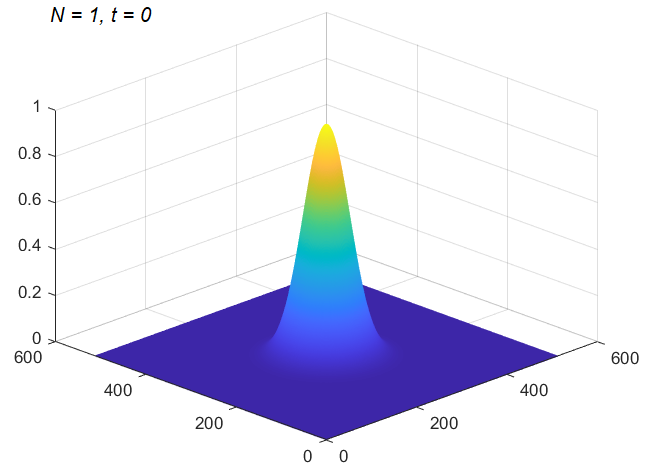
\includegraphics[scale=0.3]{Bilder_wxwy/t=0_wxwy=1_wxwy=-1}
		\end{minipage}
		\hfill 
		\begin{minipage}{0.4\textwidth}
			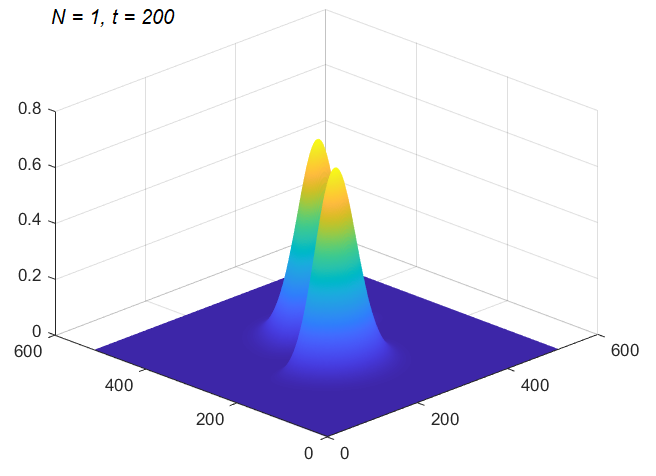
\includegraphics[scale=0.3]{Bilder_wxwy/t=200_wxwy=1_wxwy=-1}
		\end{minipage}
		\caption{Numerical results for $c^0_0$ at different times using $D_r=1$ and $w_x=w_y=1$ for $x<50$ and $w_x=w_y=-1$ otherwise. A cluster with higher particle density splits into two, each moving in opposite directions.}
		
	\begin{minipage}{0.4\textwidth}
		\centering
		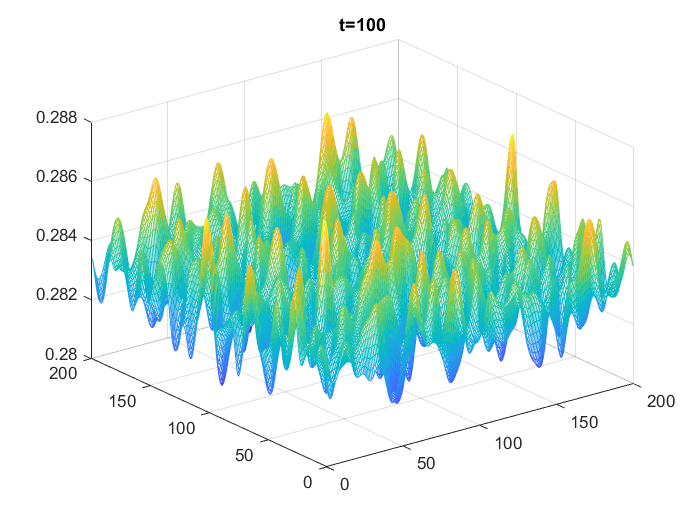
\includegraphics[scale=0.25]{Bilder_wxwy/14th_t=100_mx=my=200_random_Dr=1_(1.d0+(1.d-2rand(0)-5.d-4))Divide(2.d0dsqrt(pi))}
		\end{minipage}
		\hfill 
		\begin{minipage}{0.4\textwidth}
			\centering
			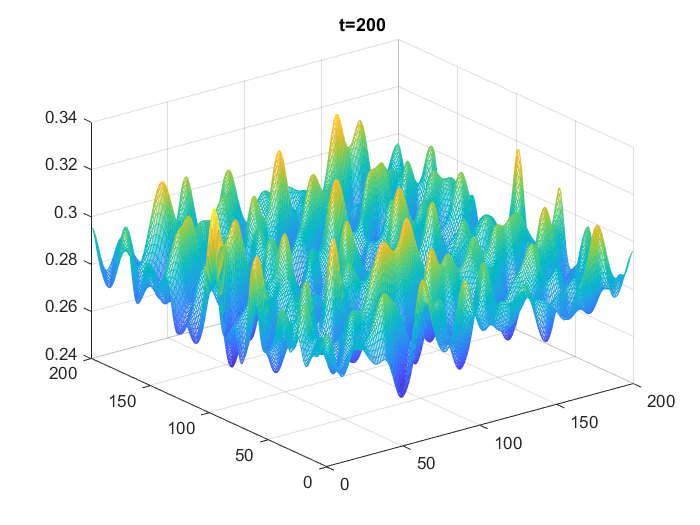
\includegraphics[scale=0.25]{Bilder_wxwy/14th_t=200_mx=my=200_random_Dr=1_(1.d0+(1.d-2rand(0)-5.d-4))Divide(2.d0dsqrt(pi))}
		\end{minipage}
		\caption{Solution structure of \(c^0_0\) with \(N = 7\).}
	\end{figure}
\end{frame}
\end{comment}









